\section{Data Analysis}
\label{sec:data_analysis}

In this section, the data collected during the experimental campaign are analyzed.
The data are processed exactly as described in the previous section (see Section \ref{sec:parameters_identification}), and the identified parameters are used to compute the numerical FRFs and so the mode shapes of the system.

In particular, by plotting the given data (which are the experimental FRFs and their coherence functions), we can clearly see that multiple peaks are present (see Figure \ref{fig:FRFs_part_B}).
However, this study will be focused on the first two peaks only, given that considering the real system from which data are acquired, those are the one of interest.

\begin{figure}[H]
    \centering
    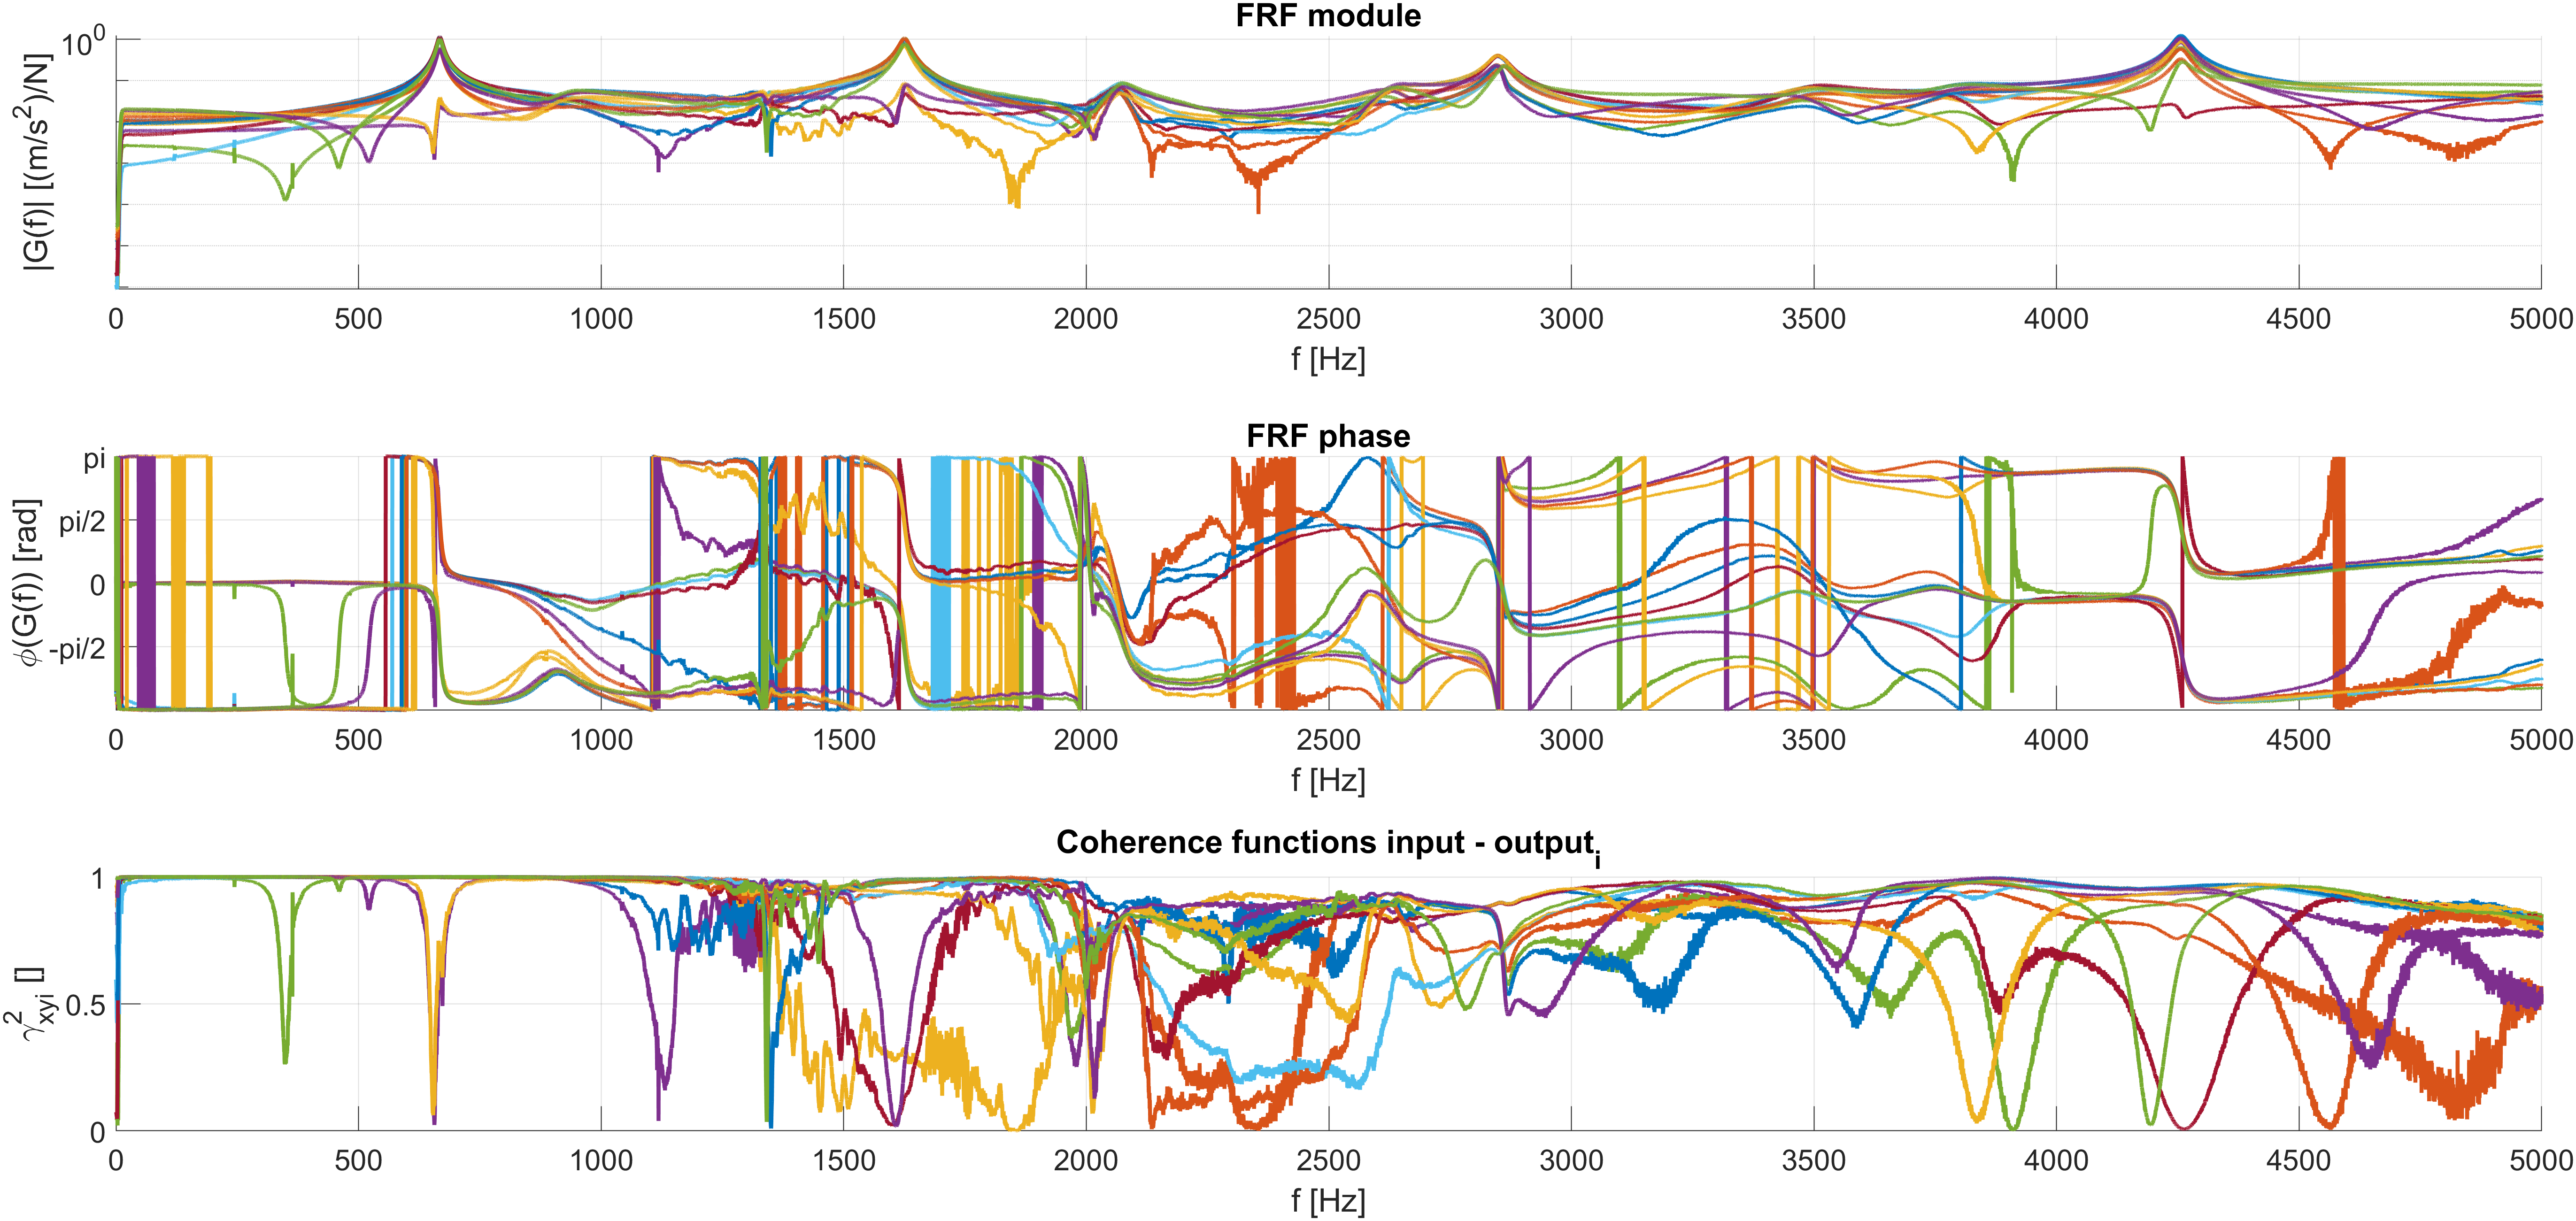
\includegraphics[width=\textwidth]{img/MATLAB/Part_B/Experimental_data.png}
    \caption{FRFs and coherence functions of the system.}
    \label{fig:FRFs_part_B}
\end{figure}


\subsection{First peak}
\label{subsec:first_peak}

Modal parameters analysis applied to the first peak of the FRFs allows us to identify the natural frequency and the damping ratio of the first mode.
The identified parameters are reported in Table \ref{tab:first_peak}.

\begin{table}[H]
    \centering
    \begin{tabular}{lc}
        \hline
        $f_i [Hz]$   & 667.324 \\
        \hline
        $\xi_i [\%]$ & 0.75 \% \\
        \hline
    \end{tabular}
    \caption{First peak modal parameters.}
    \label{tab:first_peak}
\end{table}

From a graphical point of view, the experimental and numerical FRFs are compared in Figure \ref{fig:first_peak}.


\subsection{Second peak}
\label{subsec:second_peak}

Modal parameters analysis applied to the second peak of the FRFs allows us to identify the natural frequency and the damping ratio of the second mode.
The identified parameters are reported in Table \ref{tab:second_peak}.

\begin{table}[H]
    \centering
    \begin{tabular}{lc}
        \hline
        $f_i [Hz]$ & 1625.312 \\
        \hline
        $\xi_i [\%]$       & 0.59 \%     \\
        \hline
    \end{tabular}
    \caption{Second peak modal parameters.}
    \label{tab:second_peak}
\end{table}

From a graphical point of view, the experimental and numerical FRFs are compared in Figure \ref{fig:second_peak}.
